\documentclass{article}

\usepackage[utf8]{inputenc}
\usepackage{amsmath,amssymb}
\usepackage{hyperref}
\usepackage{graphicx}

\graphicspath{ {images/} }

\author{Daniel Monjas Miguélez}
\title{Posibles Integrales Ordinaria 2021}

\begin{document}
\maketitle
\newpage

\section{Ejercicio 4. (Relación 14)}
Probar que, para cualesquiera $a,b\in \mathbb{R}^+$, se tiene:

\begin{equation*}
\int_{-\infty}^{+\infty} \frac{dx}{(x^2+a^2)(x^2+b^2)^2}=\frac{\pi (a+2b)}{2ab^3(a+b)^2}
\end{equation*}

Fijándonos en el denominador, se puede ver que tiene raíces complejas múltiples, que son $\pm ia$ simples, y $\pm ib$ dobles.

\[\int_{-\infty}^{+\infty} \frac{dx}{(x^2+a^2)(x^2+b^2)^2}=\lim_{R\to\infty}\int_{-R}^R \frac{dx}{(x^2+a^2)(x^2+b^2)^2}\]

La tarea ahora será encontrar un ciclo de manera que este contenga nuestro segmento $[-R,R]$. Hay que encontrar que la otra parte del ciclo nos de una integral muy pequeña, por ejemplo podemos tomar la semicircunferencia que parte de $R$ y termina en $R$.

\begin{figure}[h]
\centering
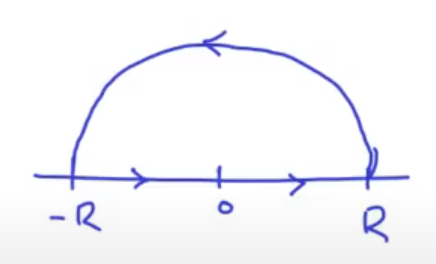
\includegraphics[scale=1,width=0.8\textwidth]{ciclo_ejer_4.png}
\end{figure}

Habrá que rodear alguna de las singularidades de nuestra función. \\

Consideramos la función $f:\Omega\backslash A\longrightarrow \mathbb{C}$, dada por $f(z)=\frac{1}{(z^2+a^2)(z^2+b^2)^2}$, donde $\Omega=\mathbb{C}$. Para poder aplicar el teorema de los residuos, el ciclo que construyamos debe ser nul-homólogo con respecto a $\Omega$, luego como $\mathbb{C}$ es homológicamente conexo tenemos una de las condiciones. Y $A=\{\pm ia,\pm ib\}$, supuesto $f\in \mathcal{H}(\Omega\backslash A)$. \\

Por otro lado, cuando $R$ creza es claro que nuestra circunferencia rodeará las singularidades. Supongamos que $a\neq b$ y tomamos $R\in \mathbb{R}^+$, con $R>max\{a,b\}$, para que así nuestra semicircunferencia contenga a $ia$ y a $ib$. Consideramos el ciclo $\Gamma_R=\sigma_R+\gamma_R$
\begin{equation*}
\left.\begin{array}{c}
\sigma_{R}:[-R,R]\longrightarrow \mathbb{C}\\
\sigma_{R}(x)=x
\end{array}\right.\qquad \left.\begin{array}{c}
\gamma_{R}:[0,\pi]\longrightarrow \mathbb{C}\\
\gamma_{R}(x)=Re^{ix}
\end{array}\right.
\end{equation*}

$\Gamma_R$ es un ciclo en $\Omega\backslash A=\mathbb{C}\backslash \{\pm ia,\pm ib\}$. Entonces tenemos que $f\in \mathcal{H}(\Omega\backslash A)$, $\Gamma_R$ es nul-homólogo con respecto a $\Omega=\mathbb{C}$ y como $A$ es finita $A'=\emptyset$, que son todas las hipótesis del teorema de los residuos, luego lo aplicamos el mismo $\Rightarrow$
\begin{gather*}
\Rightarrow \inf_{\Gamma_R}f(z)dz=2\pi i\sum_{a\in A}Ind(a)_{\Gamma_R}Res(f(z),a)=\\
=2\pi i(Ind_{\Gamma_R}(ia)Res(f(z),ia)+Ind_{\Gamma_R}(ib)Res(f(z),ib))=\\
=2\pi i(Res(f(z),ia)+Res(f(z),ib))
\end{gather*}

Por como hemos elegido el ciclo, sabemos que $Ind_{\Gamma_R}(ia)=1=Ind_{\Gamma_R}(ib)$, lo que nos permite obtener una expresión que no depende de $R$. Claramente $f$ las singularidades en $ia$ y en $ib$ son polos de orden 1.
\begin{equation*}
\int_{\sigma_R}f(z)dz+\int_{\gamma_R}f(z)dz=2\pi i(Res(f(z),ia)+Res(f(z),ib))\quad \forall R>max\{a,b\}
\end{equation*}

Entonces,
\begin{equation*}
\lim_{R\to\infty}\int_{\sigma_R}\frac{dz}{(z^2+a^2)(z^2+b^2)^2}+\lim_{R\to\infty}\int_{\gamma_R}f(z)dz=2\pi i(Res(f(z),ia)+Res(f(z),ib)) \label{(1)}
\end{equation*}

Intuitivamente sabemos que la segunda de las integrales es exactamente 0, y se comprobará ahora. Veamos que $\lim_{R\to\infty}\int_{\gamma_R}f(z)dz=0$.

Si $z\in \gamma_R^*\Rightarrow |z|=R$, y así acotamos la integral.
\begin{gather*}
|\int_{\gamma_R}f(z)dz|\leq l(\gamma_R)\frac{1}{(R^2-a^2)(R^2-b^2)^2}=\frac{\pi R}{(R^2-a^2)(R^2-b^2)^2}\left.\begin{array}{c}
R\to \infty\\
\longrightarrow 0
\end{array}\right.\\
|f(z)|=\frac{dz}{|z^2+a^2||z^2+b^2|^2}\leq \frac{1}{(R^2-a^2)(R^2-b^2)^2}\\
|z^2+a^2|\geq |z^2|-a^2=R^2-a^2>0\\
|z^2+b^2|\geq R^2-b^2>0
\end{gather*}

$\Rightarrow  \lim_{R\to\infty}\int_{\gamma_R}f(z)dz=0$. Volviendo a la igualdad \ref{(1)} tenemos la igualdad. Basta con calcular los residuos para obtener lo que nos piden.

\begin{equation*}
f(z)=\frac{1}{(z^2+a^2)(z^2+b^2)^2}=\frac{1}{(z-ia)(z+ia)(z-ib)^2(z+ib)^2}
\end{equation*}

donde vemos que $f$ tiene un polo de orden 1 en $ia$ y un polo de orden 2 en $ib$. Vamos a calcular el residuo

\begin{equation*}
\lim_{z\to ia}(z-ia)f(z)=\lim_{z\to ia}\frac{1}{(z+ia)(z^2+b^2)}=\frac{1}{2ia(b^2-a^2)^2}
\end{equation*}

Por otro lado $f$ tiene un polo de orden 2 en $ib$
\begin{gather*}
\lim_{z\to ib}\frac{\partial }{\partial z}((z-ib)^2f(z))=\lim_{z\to ib}\frac{\partial }{\partial z}(\frac{1}{(z^2+a^2)(z+ib)^2})=\\
=lim_{z\to ib}-\frac{2z(z+ib)^2+2(z^2+a^2)(z+ib)}{(z^2+a^2)^2(z+ib)^4}=\\
=lim_{z\to ib}-\frac{2z(z+ib)+2(z^2+a^2)}{(z^2+a^2)^2(z+ib)^3}=-\frac{2ib(2ib)+
2((ib)^2+a^2)}{((ib)^2+a^2)^2(2ib)^3}=\\
=\frac{4b^2+2b^2-2a^2}{-(-b^2+a^2)^28ib^3}
\end{gather*}

Sustituyendo lo anterior en la fórmula de arriba tenemos
\begin{gather*}
2\pi i(Res(f(z),ia)+Res(f(z),ib))=2\pi i\left[\frac{1}{2ia(b^2-a^2)^2}+\frac{4b^2+2b^2-2a^2}{-(-b^2+a^2)^28ib^3}\right]=\\
=\pi\left[\frac{1}{a(b^2-a^2)^2}-\frac{3b^2-a^2}{(-b^2+a^2)^22b^3}\right]=\pi\left[\frac{2b^3-3b^2a+a^3}{2b^3a(b^2-a^2)^2}\right]=\frac{\pi(a+2b)(b-a)^2}{2b^3a(b-a)^2(b+a)^2}=\\
=\frac{\pi(a+2b)}{2b^3a(b+a)^2}
\end{gather*}

\section{Ejercicio 7. Relacion 14}
Probar que, para $a,t\in\mathbb{R}^+$, se tiene:
\begin{equation*}
\lim_{R\to\infty}\int_{-R}^{R}\frac{cos(tx)}{(x^2+a^2)^2}=\int_{-\infty}^{+\infty}\frac{cos(tx)}{(x^2+a^2)^2}=\frac{\pi}{2a^3}(1+at)e^{-at}
\end{equation*}

En primer lugar es claro que el denominador de la función a integrar tiene raíces complejas dobles $\pm ia$. 

Sea $f:\Omega\backslash A\longrightarrow \mathbb{C}$ definida por
\begin{equation*}
f(z)=\frac{e^{itz}}{(z^2+a^2)^2}
\end{equation*}

, se tiene que $\Omega=\mathbb{C}$, $A=\{\pm ia\}$ y $f\in \mathcal{H}(\Omega\backslash \mathbb{C})$.

Además, ya es claro que $A'\cap \Omega=\emptyset$. También se tiene que como $\Omega =\mathbb{C}$ es homológicamente conexo entonces todo $\Gamma$ ciclo en $\Omega\backslash A$ será nul-homólogo en $\Omega$. Usando lo anterior defino el ciclo $\Gamma_R=\sigma_R+\gamma_R$, donde
\begin{equation*}
\left.\begin{array}{c}
\sigma_R:[-R,R]\longrightarrow\mathbb{C}\\
\sigma_R(z)=z
\end{array}\right.\qquad \left.\begin{array}{c}
\gamma_R:[0,\pi]\longrightarrow \mathbb{C}\\
\gamma_R(z)=Re^{iz}
\end{array}\right.
\end{equation*}

, que gráficamente es
\begin{figure}[h]
\centering
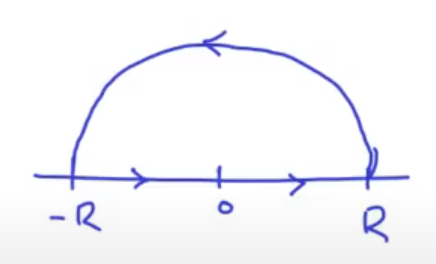
\includegraphics[scale=1,width=0.8\textwidth]{ciclo_ejer_4.png}
\end{figure}

Entonces se cumplen todas las hipótesis del teorema de residuos, y tenemos pues que
\begin{equation*}
\int_{\Gamma_R}f(z)dz=\int_{\sigma_R}f(z)dz+\int_{\gamma_R}f(z)dz=2\pi i(Ind_{\Gamma_R}(ia)Res(f(z),ia)+Ind_{\Gamma_R}(-ia)Res(f(z),-ia))
\end{equation*}

Pero los índices son claramente 1 por la elección del ciclo. Por otro lado veamos que la integral sobre la semicircunferencia se anula si $R\to\infty$.\\

En efecto,
\begin{gather*}
|\int_{\gamma_R}f(z)|\leq \pi R\frac{1}{(R^2-a^2)^2}\left.\begin{array}{c}
R\to\infty\\
\longrightarrow 0
\end{array}\right.\\
|\frac{e^{itz}}{(z^2+a^2)^2}|\leq\frac{1}{(R^2-a^2)^2}\\
|e^{itz}|=e^{-tIm(z)}\leq 1\\
|z^2+a^2|\geq |z^2|-a^2\geq R^2-a^2>0
\end{gather*}

Luego calculemos ahora los residuos. Como son dobles
\begin{gather*}
\lim_{z\to ia}\frac{\partial}{\partial z}\left(\frac{e^{itz}(z-ia)^2}{(z+ia)^2(z-ia)^2}\right)=\lim_{z\to ia}\frac{\partial}{\partial z}\left(\frac{e^{itz}}{(z+ia)^2}\right)=\\
=\lim_{z\to ia}\left(\frac{ite^{izt}(z+ia)^2-e^{itz}2(z+ia)}{(z+ia)^4}\right)=\frac{e^{-at}(2at+2)}{8ia^3}
\end{gather*}

Sustituyendo en la fórmula del teorema de residuos
\begin{equation*}
2\pi i(\frac{e^{-at}(2at+2)}{8ia^3})=\pi(\frac{e^{-at}(at+1)}{2a^3})
\end{equation*}

Ahora tomando límite en la fórmula de los residuos nos queda que
\begin{equation*}
\lim_{R\to\infty}\int_{\Gamma_R}f(z)dz=\int_{-\infty}^{+\infty}\frac{cos(tz)dz}{(z^2+a^2)^2}=\pi(\frac{e^{-at}(at+1)}{2a^3})
\end{equation*}

, pues la parte derecha de la fórmula de los residuos no depende de $R$, y la parte imaginaria de la integral de $f(z)$, se obvia, pues debe ser 0, pues la parte de los residuos es completamente real


\section{Ejercicio 14. Relación 4}
Integrando una conveniente función sobre la poligonal $[-R,R,R+\pi i,-R+\pi i,-R]$, con $R\in \mathbb{R}^+$, calcular la integral
\begin{equation*}
\int_{-\infty}^{+\infty}\frac{\cos{x}}{e^x+e^{-x}}
\end{equation*}

Fijamos $R>0$ y consideramos la función 
\begin{gather*}
f:\mathbb{C}\backslash A\longrightarrow \mathbb{C}\\
f(z)=\frac{e^{iz}}{e^z+e^{-z}}\\
e^z+e^{-z}=0\Leftrightarrow e^{2z}+1=0\Leftrightarrow e^{2z}=-1\Leftrightarrow 2z\in Log(-1)=ln|-1|+iArg(-1)\Leftrightarrow\\
\Leftrightarrow 2z\in i(\pi + 2\pi \mathbb{Z})\Leftrightarrow z\in i(\frac{\pi}{2}+\pi\mathbb{Z})
\end{gather*}

, luego $A=i(\frac{\pi}{2}+\pi\mathbb{Z})$, y $f\in \mathcal{H}(\mathbb{C}\backslash  A)$. Fijándonos en que $A'=\emptyset$ aunque sea infinito y que $\Gamma_R=[-R,R,R+\pi i,-R+\pi i,-R]$ es un ciclo en $\mathbb{C}\backslash A$ nul-homologo respecto a $\mathbb{C}$, pues $\mathbb{C}$ es homológicamente conexo. Luego podemos aplicar el teorema de los residos, de forma que
\begin{equation*}
\int_{\Gamma_R}f(z)dz=2\pi Ind_{\Gamma_R}(\frac{i\pi}{2})Res(f(z),\frac{i\pi}{2})
\end{equation*}

, donde es claro que ese índice es 1, pues sólo se da una vuelta en el rectángulo alrededor del punto. Por otro lado es claro que se verifica que
\begin{equation*}
\int_{\Gamma_R}f(z)dz=\int_{[-R,R]}f(z)dz+\int_{[R,R+\pi i]}f(z)dz+\int_{[R+\pi i,-R+\pi i]}f(z)dz+\int_{[-R+\pi i,-R]}f(z)dz
\end{equation*}
\end{document}